\documentclass[
    a4paper,
    12pt,
    fleqn,
    twoside
]{report}
\usepackage{duarte}
\usepackage{blindtext}
% ----------------------------
\begin{document}

% ============================
% CAPA
\begin{titlepage}
    \begin{center}
     {\LARGE \bfseries SÃO PAULO STATE UNIVERSITY}
     
     {\LARGE School of Engineering of Ilha Solteira}
     
     \vfill
     
     {\Huge \bfseries TITLE}
     
     \vfill
     
     \includegraphics[width=0.7\textwidth]{figures/logos/gmsint_logo_new.pdf}
     
     \vfill
     
     \begin{minipage}{0.7\textwidth}
      {\large \bfseries Research Report -- Iniciação Científica}
      
      {\large \bfseries Student: Gabriel D. Silva}
      
      {\large Professor: Douglas D. Bueno}
      
     \end{minipage}
     
     \vfill
     
     {\large \bfseries UNESP}
     
     {\large \bfseries Ilha Solteira -- SP}
     
     {\large \bfseries 2022}
    \end{center}
   \end{titlepage}
% ----------------------------

% ============================
% RELATÓRIO DE PESQUISA
\setcounter{page}{1}
\pagenumbering{roman}
\pagestyle{empty}
\begin{center}
	\vspace{100pt}
	{\Large\sffamily\bfseries RESEARCH REPORT}
\end{center}
\noindent
Lorem ipsum dolor sit amet, consectetur adipiscing elit. Ut pulvinar rhoncus dapibus. In orci odio, elementum vitae eros nec, rhoncus mattis ante. Proin vitae magna feugiat, facilisis enim nec, faucibus ante. Nullam rhoncus est ac odio sodales, et congue purus varius. Pellentesque nec ligula ante. Nunc volutpat nunc sit amet leo tempor consequat. Nulla et lectus id nisl pharetra aliquet ac quis tellus. Integer quis dictum nibh. Morbi ut nunc a quam fringilla commodo nec vitae tellus. Suspendisse tristique vel nisl vitae ornare. Aliquam a imperdiet dui. Phasellus a rhoncus mi. Quisque condimentum lacus velit, quis aliquet risus cursus non.


\noindent
{\bfseries Keywords:} word, word, word.

\clearpage
% ----------------------------

% ============================
% LISTA DE FIGURAS
{\sffamily\listoffigures}
\newpage
% ----------------------------

% ============================
% LISTA DE TABELAS
% {\sffamily\listoftables}
% \newpage
% ----------------------------

% ============================
% LISTA DE ABREVIAÇÕES
\setlist[description]{leftmargin=!, labelwidth=3em} % Change for glossaries
\printglossary[title={List of Abbreviation}, nonumberlist]
\setlist[description]{style=standard} % reset settings back to default
\newpage
% ----------------------------

% ============================
% SUMÁRIO
{\sffamily\tableofcontents}
\newpage
% ----------------------------

% ============================
% FORMATAÇÕES EXTRAS
\setcounter{page}{1}
\pagenumbering{arabic}
\pagestyle{fancy}
% ----------------------------

% ============================
% SEÇÕES
\chapter{Results and Discussion}\label{sec:results}

% \begin{figure}
%     \centering
%     \import{/home/gabriel/Documentos/deep-learning/report/figures/}{plot_style.pgf}
% \end{figure}

\chapter{Results and Discussion}\label{sec:results}

% \begin{figure}
%     \centering
%     \import{/home/gabriel/Documentos/deep-learning/report/figures/}{plot_style.pgf}
% \end{figure}
\section{Structural Health Monitoring}

\subsection{Definition}

According to  \citet{balageas2010}, the \gls*{shm} main purpose is to provide, during the life of a structure,  a diagnosis of: the state of the constituent material; the different parts of the structure; and the full assembly of each part that makes the structure as a whole. 
It is an improved way to make non-destructive evaluation.
It can be applied in several areas such as civil infrastructure, like bridges and buildings; aerospace, like airplanes and spaceships; and mechanical, like machines.

\begin{figure}[H]
    \centering
    \includegraphics[width=0.6\textwidth]{figures/2methodology/shm/smh_nervous_system.png}
    \caption[SHM and human nervous system analogy]{\gls*{shm} and human nervous system analogy. Source: \citet{blanckenstein2015}}
    \label{fig:shm_nervous_system}
\end{figure}

It also can be associated as an analogy to the human nervous system, as shown in the \cref{fig:shm_nervous_system}. Just like the sensors send a signal to the central processor, the human 
senses send a signal to the brain to make the recognition of what is happening.

\subsection{Brief History}

The history goes back to the 1960s, when researches\(\ldots\) 

\begin{equation}
    \mathcal{L}\{f(x)\} = \lim_{\theta\to 0^+} \int_{\theta}^{\infty} f(x)\,\exp(-st) \, dt
\end{equation}
\section{Study Case 1: Unnamed Aerial Vehicle}

\subsection{Model Summary}

After the \gls*{nn} training, it was tested using the 200 samples, as the~\cref{tab:ann_parameters_uav}.
The metrics to evaluate the model are shown in the~\cref{tab:model_summary_uav}.
%
\begin{table}[!htb]
    \centering
    \caption{Model summary}
    \begin{tblr}{
        row{even}={light_color}
    }
    \toprule
    Parameter & Value \\
    \midrule
    MSE & 0.00085 \\
    MAE & 0.00746 \\
    \bottomrule
    \end{tblr}

    {\footnotesize Source: prepared by the author.}
    \label{tab:model_summary_uav}
\end{table}

\begin{figure}[!htb]
    \centering
    \caption{Some caption}
    \import{/home/gabriel/Documentos/deep-learning/report/figures/4results/uav/}{epochsxloss.pgf}
\end{figure}

\subsection{Comparison of the Model with the Script}

The~\cref{fig:uxt_comparison_model_script} shows the comparison of the control torque from the script with the \gls*{nn} created model for the same \(\symbf{x}_s\).
%
\begin{figure}[!htb]
    \centering
    \caption[Comparing the model with the script]{Comparing the model with the script. The continuous curve is the control torque from the script, while dashed curve is the output from the \gls*{nn} model.}
    \import{/home/gabriel/Documentos/deep-learning/report/figures/4results/uav}{uxt_comparasion_model_script.pgf}

    {\footnotesize Source: prepared by the author.}
    \label{fig:uxt_comparison_model_script}
\end{figure}

From the model statistics, the loss function for the test sample gave the result of 0.00085, which is an acceptable value for its purpose.
Although the~\cref{fig:uxt_comparison_model_script} looks like to show some discrepancy for \(U_2(t)\) and \(U_3(t)\), they do not mean the model did not predict precisely the control torque. 
After the first 10 seconds, which is the time that the \gls*{uav} is leaving the ground, the model is able to describe the control torque very well.

The major error, i.e., in the beginning of the motion may be caused by the interference of the \(z\)-axis trajectory. 
The discrepancy, actually, represents very little in the major context, since the image scale may distort the real values.
That said, other possible reason for the error in the model is the quantity of samples to make the training of the neural network. 
A thousand trajectories is not a good quantity for the model to make a good prediction.
To have an accurate model, it should have at least one hundred thousand trajectories, but due to the processing limitation, it was not possible.

Even though the model curve did not overlap the curve from the script, it gave the same pattern.
\section{Neural Networks}

\subsection{Deep Learning}

The concepts of deep learning studied in this section is going to be based on the work of \citet{goodfellow2016}.

There are several definitions of \gls*{ai} \citep{winston1992}, but the  computer scientist \citet{mccarthy2007} defines it as ``the science and engineering of making intelligent machines, especially intelligent computer programs.''.
He also states that ``it is related to the similar task of using computers to understand human intelligence, but AI does not have to confine itself to methods that are biologically observable.''.

The big area of study is the \gls*{ai} and it includes several branches like fuzzy logics, robotics, machine learning and so on. 
The later one, in turn, is another field with also some branches and one of them is the deep learning.
This can be represented in a Venn diagram, as the \cref{fig:venn_dl} shows.
However, all the three terms can be interchangeable in the major context.

\begin{figure}[H]
    \centering
    
\includegraphics{figures/2methodology/nn/venn_dl.pdf}
    \caption{Subareas of Artificial Intelligence}
    \label{fig:venn_dl}
\end{figure}

The deep learning history goes back to the 1940s and it had several names over the years. It was called by \emph{cybernetics} (1940s--1960s), \emph{connectionism} (1980s--1990s), and from 2006 until now is known as \emph{deep learning}.
The \gls*{dl} models were engineered systems inspired by the biological brain and they were denominated \gls*{ann}.
One of the motivations of the neural perspective was to understand that the brain provides a proof by example that intelligent behavior is possible and try to reverse engineer the computation principals behind the brain, duplicating its functionality.

\gls*{dl} today goes beyond the neuroscientist perspective and it is more of general principle of learning multiple levels of composition.

\subsection{Multilayer Perceptron}

A \gls*{mlp}, also known as \emph{deep network}, is the essence of \gls*{dl}. Basically, it is a mathematical function, formed by composing many simpler functions, mapping some set of input values to output values.
%
\begin{figure}[H]
    \centering
    \includegraphics{figures/2methodology/nn/mlp.pdf}
    \caption[Multilayer Perceptron Scheme]{Multilayer Perceptron Scheme. It resembles a human neuron: input layer data is equivalent to the dendrites; hidden layers are the equivalent of the axons; and the output layer are the equivalent of the nerve ending. The figure show two hidden layers, but it can contain multiple of them.}
\end{figure}

\noindent\textcolor{red}{PUT THE FORMULAS OF HOW MLP WORKS.}
\section{Algorithm Implementation}

\subsection{MATLAB Algorithm to Determine the Forces}

\subsection{PyTorch Algorithm to Detect Railway Cracks}

\chapter{Results and Discussion}\label{sec:results}

% \begin{figure}
%     \centering
%     \import{/home/gabriel/Documentos/deep-learning/report/figures/}{plot_style.pgf}
% \end{figure}

\chapter{Results and Discussion}\label{sec:results}

% \begin{figure}
%     \centering
%     \import{/home/gabriel/Documentos/deep-learning/report/figures/}{plot_style.pgf}
% \end{figure}
% ----------------------------

% ============================
% REFERÊNCIAS
% \printbibliography
\bibliographystyle{chicago}
\bibliography{ref}
% ----------------------------

% ============================
% APÊNDICE
\appendix
\titleformat{\chapter}{\sffamily\centering\bfseries\large}%
{APPENDIX \thechapter \,--}{1mm}{\large}

% ============================
% RELATÓRIO DE PESQUISA
\end{document}